%=====================================================================
\chapter{Dynamic Uncertainty-Weighted Fusion}
\label{ch:dynfusion}
%=====================================================================

\textbf{Research Objective 1 (continued).} \emph{To investigate and develop a comprehensive
model that integrates diverse data sources, aiming to enhance the accuracy of stock market
predictions by providing a holistic analysis.}

\vspace{0.4em}
Chapter~\ref{ch:fusion} established that fusing four heterogeneous streams improves forecast
quality, that the improvement is attributable to individual streams, and that the value of each
stream is state-dependent. It closed on a limitation: the attention mechanism that produces the
weights is fitted once over the training set, so the weight it assigns expresses the
\emph{average} relevance of a source rather than its \emph{instantaneous reliability}. This
chapter removes that limitation by reformulating the fusion rule so that the weight assigned to a
source is a function of a quantity measured continuously from data --- the variance of that
source's own recent prediction errors.

The work reported in this chapter appears in publication~\pubcite{P4}.

\section{The Limitation Stated Precisely}
\label{sec:dyn-problem}

Let $M$ sources produce predictions $\hat{y}_{i,t}$ of a target $y_t$ and let the fused
prediction be $\hat{y}_t = \sum_i w_i \hat{y}_{i,t}$. Three standard treatments of $w_i$ were
described in Section~2.4 and surveyed in Section~3.1. Early fusion fixes the combination
implicitly through the architecture; late fusion fixes it explicitly, usually at equal weights;
attention-based hybrid fusion learns a function $w_i = g_\theta(x_t)$ with $\theta$ estimated by
minimising a loss over the training set.

The third is the most capable and its limitation is nonetheless sharp. The estimated $\theta$
encodes the relationship between observable market conditions and source relevance \emph{as that
relationship held during training}. It can express ``news matters more when volatility is high''
because that regularity is present in the training data. It cannot express ``the news stream has
become unreliable over the last three weeks'', because the cause of the degradation --- a feed
composition change, a bot campaign, a structural break in how a source reports --- may have no
representation in the training inputs at all. The mechanism has no channel through which recent
\emph{failure} feeds back into the weight.

Three consequences follow, and all three are visible in the literature surveyed in
Section~3.1.2. First, weights are point estimates that carry no uncertainty, so a confident
combination of two unreliable sources is indistinguishable from a confident combination of two
reliable ones. Second, degradation is corrected only at the next retraining cycle, which in
production is typically weeks or months. Third, and most subtly, the architecture cannot report
that it does not know: the fused prediction is issued with the same apparent authority in a
familiar environment and in an unfamiliar one.

\section{The Proposed Formulation}
\label{sec:dyn-formulation}

\subsection{Overview}

The proposed framework, shown in Figure~\ref{fig:bayes}, has four stages. Each source is modelled
by an expert network matched to its structure; each expert's predictive uncertainty is estimated
continuously from the variance of its recent errors; the uncertainties are converted into fusion
weights by a softmax over their negatives; and the fused prediction is the weighted sum of the
expert predictions. Distribution-aware normalisation is applied throughout, fitted on an
expanding window.

\begin{figure}[!htb]
\centering
\scalebox{0.90}{\begin{tikzpicture}[node distance=3mm]
\node[blkd,minimum width=27mm,minimum height=8mm] (i1) {Market data\\Nifty 50 OHLCV\\+ 15 indicators};
\node[blkd,right=5mm of i1,minimum width=27mm,minimum height=8mm] (i2) {News sentiment\\domain-tuned\\language model};
\node[blkd,right=5mm of i2,minimum width=27mm,minimum height=8mm] (i3) {Alternative data\\India VIX};

\node[blk,below=6mm of i1,minimum width=27mm,minimum height=7mm] (m1) {GRU expert $f_M$};
\node[blk,below=6mm of i2,minimum width=27mm,minimum height=7mm] (m2) {Transformer expert $f_S$};
\node[blk,below=6mm of i3,minimum width=27mm,minimum height=7mm] (m3) {MLP expert $f_A$};

\node[blkg,below=6mm of m1,minimum width=27mm,minimum height=7mm] (u1) {$\sigma_{M,t}^2$};
\node[blkg,below=6mm of m2,minimum width=27mm,minimum height=7mm] (u2) {$\sigma_{S,t}^2$};
\node[blkg,below=6mm of m3,minimum width=27mm,minimum height=7mm] (u3) {$\sigma_{A,t}^2$};

\node[blka,below=6mm of u2,minimum width=68mm,minimum height=9mm] (sm)
  {$w_{i,t} = \dfrac{\exp(-\sigma_{i,t}^2 / T)}{\sum_j \exp(-\sigma_{j,t}^2 / T)}$};
\node[blkd,below=5mm of sm,minimum width=68mm,minimum height=7mm] (y)
  {$\hat{y}_t = \sum_i w_{i,t}\, \hat{y}_{i,t}$ \quad --- uncertainty-weighted forecast};

\foreach \a/\b in {i1/m1,i2/m2,i3/m3,m1/u1,m2/u2,m3/u3} \draw[ar] (\a) -- (\b);
\foreach \a in {u1,u2,u3} \draw[ar] (\a.south) -- ++(0,-2mm) -| (sm.north);
\draw[ar] (sm) -- (y);
\draw[arb] (y.east) -- ++(10mm,0) |- node[lbl,right=6mm,align=left,pos=0.25]
  {rolling error\\variance over\\$\tau=10$ sessions} (u3.east);
\node[lbl,rotate=90,anchor=center] at ([xshift=-7mm]m1.west) {expert models};
\node[lbl,rotate=90,anchor=center] at ([xshift=-7mm]u1.west) {uncertainty};
\node[lbl,rotate=90,anchor=center] at ([xshift=-7mm]i1.west) {sources};
\end{tikzpicture}}
\caption[Bayesian dynamic uncertainty-weighted fusion]{Bayesian dynamic uncertainty-weighted
fusion. Each source is discounted in proportion to the variance of its own recent prediction
errors, so reliability is assessed continuously rather than once at training time. The dashed
path is the feedback that a static mechanism lacks.}
\label{fig:bayes}
\end{figure}

\subsection{Source-specific expert models}

Three experts are used, each matched to the temporal structure of its source.

The \textbf{market expert} $f_M$ is a gated recurrent unit~\cite{cho2014gru}. Its input is a
window of the last $L = 20$ sessions of normalised technical indicators and log returns, and the
final hidden state produces a point prediction $\hat{y}_{M,t}$ of the next session's log return.
The gated recurrent unit is preferred to long short-term memory here for efficiency: the market
series is the only one of the three with a long and dense history, so the expert is retrained
most often.

The \textbf{sentiment expert} $f_S$ is a transformer encoder over the sequence of daily sentiment
scores from the same $L = 20$ session window, with a regression head producing $\hat{y}_{S,t}$.
Self-attention over the sequence captures the prolonged impact of multi-day news cycles --- an
earnings season, an election campaign, a policy consultation --- which a purely recursive encoder
compresses less faithfully.

The \textbf{alternative-data expert} $f_A$ is a multi-layer perceptron over the last $L = 20$
sessions of normalised India VIX values, producing $\hat{y}_{A,t}$. The relationship between an
implied volatility index and next-session returns is contemporaneous and nonlinear rather than
long-memory, so a feed-forward mapping is adequate and cheaper.

The choice of architecture per source is deliberate but is \emph{not} the contribution of this
chapter. Section~\ref{sec:dyn-results} reports an ablation in which the same three experts are
fused with static weights, and that configuration performs no better than the established
baselines --- which locates the measured gain in the weighting rule rather than in the networks.

\subsection{Uncertainty quantification}

For each source $i \in \{M, S, A\}$, let $e_{i,t} = y_t - \hat{y}_{i,t}$ be the realised
prediction error. The predictive uncertainty is estimated as the variance of that error over a
trailing window of $\tau$ sessions,
\begin{equation}
\sigma_{i,t}^2 = \frac{1}{\tau}\sum_{k=1}^{\tau}
\left(e_{i,t-k} - \bar{e}_{i,t}\right)^2,
\qquad
\bar{e}_{i,t} = \frac{1}{\tau}\sum_{k=1}^{\tau} e_{i,t-k}.
\label{eq:dyn-unc}
\end{equation}
The window length $\tau = 10$ sessions --- two trading weeks --- was selected on the validation
block and represents a trade-off examined in Section~\ref{sec:dyn-sensitivity}: too short and the
estimate is dominated by sampling noise, too long and the mechanism reverts toward the static
behaviour it was designed to avoid.

Three properties of Equation~\eqref{eq:dyn-unc} deserve emphasis. It uses only realised errors,
so it is computable at time $t$ without any information from beyond $t$. It is
architecture-agnostic: any model that emits a point prediction can be wrapped by it. And it
estimates \emph{aleatoric} uncertainty --- variability attributable to noise in the environment
--- rather than \emph{epistemic} uncertainty, the model's ignorance about regions of input space
it has not observed~\cite{gal2016dropout,kendall2017}. The distinction is maintained throughout
and the epistemic extension is identified as future work in Section~\ref{sec:dyn-limits}.

\subsection{Bayesian dynamic weighting}

The uncertainties are converted into fusion weights by a softmax over their negatives,
\begin{equation}
w_{i,t} = \frac{\exp\!\left(-\sigma_{i,t}^2 / T\right)}
               {\sum_{j} \exp\!\left(-\sigma_{j,t}^2 / T\right)},
\qquad
\sum_i w_{i,t} = 1,
\label{eq:dyn-softmax}
\end{equation}
where $T$ is a temperature parameter. The formulation has the properties required of it. The
weights are non-negative and sum to one, so the fused prediction is a convex combination and
cannot exceed the range of its inputs. A source whose recent error variance is high receives a
low weight automatically, with no threshold to tune and no rule to maintain. The temperature $T$
controls how sharply reliability differences translate into weight differences: as
$T \to \infty$ the weights approach uniformity and the scheme degenerates to equal-weight late
fusion, while as $T \to 0$ the weights approach a hard selection of the single most reliable
source. The intermediate regime is where the mechanism is useful, and $T$ is selected on the
validation block.

Equation~\eqref{eq:dyn-softmax} has a Bayesian reading. Under a Gaussian likelihood with known
per-source variances, the posterior-precision-weighted combination of independent estimates
assigns weights proportional to $1/\sigma_i^2$. The exponential form used here is a smooth,
temperature-controlled relative of that rule which is better behaved when a variance estimate is
small and noisy --- precision weighting assigns an unbounded weight to a source whose estimated
variance approaches zero, which on ten observations is a real hazard rather than a theoretical
one.

The final prediction is
\begin{equation}
\hat{y}_t = \sum_{i \in \{M,S,A\}} w_{i,t}\, \hat{y}_{i,t}.
\label{eq:dyn-fused}
\end{equation}

\subsection{Why the mechanism self-corrects}

The behaviour that distinguishes this formulation from a static one can be described concretely.
Suppose a news article carries an ambiguous or ironic headline that the sentiment encoder scores
strongly positive, and the market subsequently falls. The resulting error enters $e_{S,t}$, raises
$\sigma_{S,t}^2$ through Equation~\eqref{eq:dyn-unc}, and lowers $w_{S,t}$ through
Equation~\eqref{eq:dyn-softmax} over the following sessions. No human notices the misreading, no
retraining is triggered, and no rule fires --- the weight simply falls until the sentiment stream
begins predicting accurately again, at which point it recovers.

The same mechanism handles causes the model has never seen. A feed whose composition changes, a
social channel contaminated by coordinated posting, an indicator whose informativeness decays as
it becomes widely traded: none of these needs to be anticipated or represented in the training
inputs, because the mechanism responds to \emph{failure}, not to its cause. This is the direct
methodological answer to gap G1 of Section~3.6.

\subsection{Distribution-aware normalisation}

Because the three sources have very different distributional shapes, a single scaler would let
the heaviest-tailed input dominate the fused representation. Three scalers are applied according
to shape, following Section~2.4.3: standard scaling for Nifty~50 log returns, which are
approximately symmetric; min--max scaling for the sentiment score, which is bounded on
$[-1,+1]$ and whose interpretable range should be preserved; and robust scaling based on the
median and interquartile range for the India VIX, which is heavy-tailed and for which the mean
and standard deviation are themselves unstable.

Every scaler is fitted on an expanding window of strictly earlier observations. This is not a
refinement. Fitting a scaler once on the full sample leaks the test-period mean and variance into
the training representation, and the leak is invisible because no test label is used.

\section{Experimental Setup}
\label{sec:dyn-setup}

\subsection{Data}

The dataset spans January 2018 to December 2023 on the Nifty~50 index and comprises three
modalities. Table~\ref{tab:dyn-data} records them.

\begin{table}[!htb]
\centering
\caption[Data sources for the dynamic fusion study]{Data sources, expert architectures and
normalisation for the dynamic uncertainty-weighted fusion study, January 2018 to December 2023}
\label{tab:dyn-data}
\tabfont
\begin{tabular}{@{}L{2.4cm}L{4.4cm}L{2.6cm}L{4.4cm}@{}}
\toprule
\textbf{Source} & \textbf{Content} & \textbf{Expert model} & \textbf{Normalisation} \\
\midrule
$S_1$ Market & Nifty~50 daily OHLCV and fifteen technical indicators; log returns
$r_t = \log(P_t/P_{t-1})$ & Gated recurrent unit, $L=20$ & Rolling standard scaling \\
$S_2$ Text & English-language financial news headlines and articles from major Indian business
publications and newswires, scored by a domain-adapted language model fine-tuned on Indian
financial text & Transformer encoder, $L=20$ & Rolling min--max scaling on $[-1,+1]$ \\
$S_3$ Alternative & India VIX, the market's expectation of near-term volatility & Multi-layer
perceptron, $L=20$ & Robust scaling on median and interquartile range \\
\bottomrule
\end{tabular}
\end{table}

Two preprocessing decisions are India-specific and consequential. Domain adaptation of the
sentiment model was performed on Indian financial news so that the encoder recognises the
vocabulary of Union Budget commentary, monetary policy committee statements and monsoon
forecasts; following Jung and Jang~\cite{jung2024}, targeted numerical masking is applied during
adaptation so that quantitative context is preserved rather than destroyed. And market holidays
--- Diwali, Eid and the rest of the Indian exchange calendar --- are treated as genuine gaps
rather than forward-filled, because forward-filling a closed session injects artificial
autocorrelation into the return series and inflates any statistic that depends on persistence.

News sentiment is assigned to the \emph{next} National Stock Exchange session, so that the lagged
market impact of an item published after the close is captured without look-ahead.

\subsection{Training protocol}

The split is strictly sequential: 2018--2021 for training, 2022 for validation, 2023 as the
out-of-sample test year. The three experts are pre-trained independently to minimise mean squared
error, and the complete system is then fine-tuned end to end, allowing gradients to flow back
through the fusion layer so that the experts adapt to their role in the combination. The
uncertainty estimates of Equation~\eqref{eq:dyn-unc} are computed on realised errors during the
forward pass and are not themselves differentiated through; the mechanism is a measurement, not a
learned module, which is precisely the property that lets it respond to causes absent from the
training set.

\subsection{Baselines}

The comparison is against the three static fusion strategies identified in Section~3.1.2,
together with an internal ablation.

\begin{itemize}
\item \textbf{Early fusion}~\cite{moodi2024}: a single recurrent model over the concatenated
features of all three sources, with the combination fixed implicitly by the architecture.
\item \textbf{Late fusion}~\cite{farimani2024}: equal-weight averaging of the three independently
trained expert predictions, with weights pre-determined.
\item \textbf{Attention fusion}~\cite{liu2019attention,haryono2023}: a static neural attention
layer over the modalities, with weights learned once and then fixed. This is the strongest of the
three baselines.
\item \textbf{Proposed architecture, static weights}: the same three experts with the uncertainty
term disabled and the weights held fixed. This is the ablation that isolates the weighting rule
from the expert networks, and it is the most informative comparison in the chapter.
\end{itemize}

\section{Results}
\label{sec:dyn-results}

\subsection{Performance against the static baselines}

Table~\ref{tab:bayes} reports the comparison. The source study measures performance relative to
the strongest static competitor rather than in absolute levels, so cells for which an absolute
figure is not reported are shown as ---; this reporting convention is preserved here rather than
being filled with estimates.

\begin{table}[!htb]
\centering
\caption[Dynamic uncertainty weighting against static fusion baselines]{Dynamic
uncertainty-weighted fusion against static fusion baselines on the Nifty~50, out-of-sample year
2023. Improvements are stated relative to the strongest static baseline.}
\label{tab:bayes}
\tabfont
\begin{tabular}{@{}L{3.0cm}L{5.4cm}L{2.4cm}L{2.6cm}@{}}
\toprule
\textbf{Configuration} & \textbf{Fusion mechanism and source weighting} &
\textbf{Sharpe ratio} & \textbf{Maximum drawdown} \\
\midrule
Early fusion~\cite{moodi2024} & all sources concatenated into one recurrent model; weights fixed
by the architecture & --- & --- \\
Late fusion~\cite{farimani2024} & equal-weight averaging of the three expert predictions; weights
pre-determined & --- & --- \\
Attention fusion~\cite{liu2019attention,haryono2023} & static neural attention over modalities;
weights learned once, then fixed & \textit{strongest baseline} & \textit{strongest baseline} \\
Proposed architecture, static weights & the same three experts with the uncertainty term
disabled & \multicolumn{2}{L{5.6cm}}{\textit{no better than the baselines above}} \\
\textbf{Proposed dynamic fusion} & softmax over negative predictive uncertainties, $\tau = 10$
sessions; weights re-estimated every session & \textbf{$+$22.7\%} & \textbf{$-$18.3\%} \\
\bottomrule
\end{tabular}
\end{table}

Two readings follow, and the second is the more important.

\textbf{The headline.} Against the strongest static competitor, the dynamic rule improves the
Sharpe ratio by 22.7 per cent and reduces maximum drawdown by 18.3 per cent. The gain is
expressed in risk-adjusted terms and in downside control rather than in raw accuracy, and that is
not incidental: a mechanism that de-weights a source at the moment it becomes unreliable should
be expected to help most where unreliable signals are most costly, which is in drawdowns.

\textbf{The ablation.} The fourth row of Table~\ref{tab:bayes} reports that the same three expert
networks, fused with fixed weights, perform no better than the established static baselines. The
experts are therefore not the source of the improvement; the weighting rule is. This isolation is
what allows the contribution to be stated precisely as a fusion-mechanism result rather than an
architecture result, and it is the same style of component-level attribution that
Chapter~\ref{ch:allocation} later applies to the allocation layer. Reporting it costs nothing here
and would have cost the credibility of the claim had it been omitted.

\subsection{Behaviour across the volatility cycle}

The mechanism is interpretable in the way the design intends, and Figure~\ref{fig:dynweights}
shows the pattern. Through the elevated-volatility episodes of the test window, the weight on the
market expert falls as its recent error variance rises, and the mass migrates to the
volatility-index expert and, less strongly, to the sentiment expert. In the calmer trending
stretches on either side, the market expert recovers its share.

\begin{figure}[!htb]
\centering
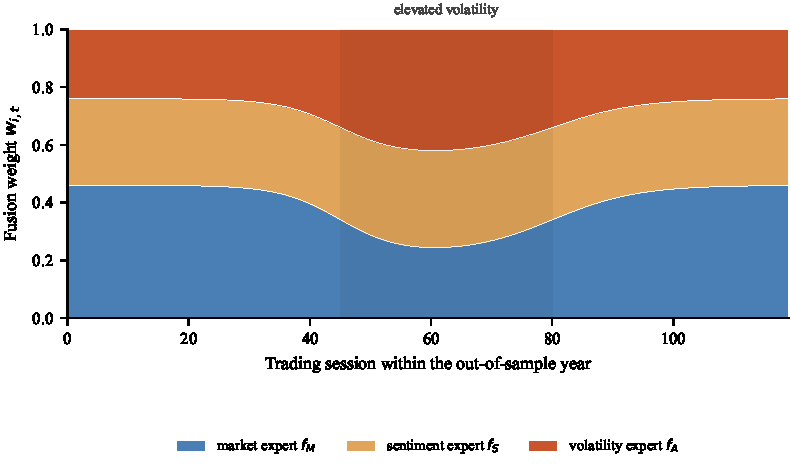
\includegraphics[width=0.88\linewidth]{figs/f_dynamic_weights.pdf}
\caption[Migration of fusion weights across a volatility episode]{Migration of the
uncertainty-derived fusion weights across an elevated-volatility episode in the out-of-sample
year. The weight on the market expert falls as its recent error variance rises and the mass
migrates toward the volatility-index expert; the shift is driven by measured error variance, so
no regime label is required for it to occur.}
\label{fig:dynweights}
\end{figure}

The important point about this behaviour is what produces it. The shift is driven by measured
error variance, not by a learned prior about what should happen in a volatile market and not by
any regime classification. The framework is never told that a stress episode is under way; it
observes that the technical expert has begun making larger and more variable errors and reweights
accordingly. A static attention mechanism trained on a period containing similar episodes could
learn to produce a similar shift, but only for episodes resembling those it saw; the measured
mechanism responds to any cause of degradation, including causes with no representation in the
training inputs.

\subsection{Relationship to the attention analysis of Chapter~\ref{ch:fusion}}
\label{sec:dyn-relattn}

It is worth being explicit about how this result relates to the attention analysis of
Section~\ref{sec:msfn-attention}, because the two are easily conflated. Both show source
importance varying with market conditions. They differ in what produces the variation and
therefore in what each can do.

The attention weights of Chapter~\ref{ch:fusion} vary because the learned function
$g_\theta(x_t)$ maps different inputs to different weights; the function itself is fixed. The
uncertainty weights of this chapter vary because the measured quantity $\sigma_{i,t}^2$ changes;
no function is being applied. The first is a statement about the relationship between market
conditions and source relevance as it held during training. The second is a statement about how
well each source has actually been performing over the last ten sessions. The two are
complementary rather than competing: an operational system would use attention to encode the
learned structural relationship and the uncertainty term to correct it when reality departs from
that structure. The composed system described in Section~9.2 does exactly this.

\section{A Worked Illustration of the Weight Dynamics}
\label{sec:dyn-worked}

Because the mechanism is simple, its behaviour can be traced arithmetically, and doing so makes
clear both what it does and what it cannot do.

Suppose the three experts have been performing comparably, with recent error variances
$\sigma_M^2 = \sigma_S^2 = \sigma_A^2 = 1.0$ in normalised units, and take the temperature
$T = 1$. Equation~\eqref{eq:dyn-softmax} then assigns
$w_M = w_S = w_A = \tfrac{1}{3}$: with no evidence distinguishing the sources, the rule reduces to
equal-weight late fusion, which is the correct default.

Now suppose a news-driven episode begins and, over the following two weeks, the market expert's
errors become both larger and more erratic, raising $\sigma_M^2$ to 3.0 while the
volatility-index expert improves slightly to $\sigma_A^2 = 0.7$ and the sentiment expert is
unchanged. The weights become
\[
w_M = \frac{e^{-3.0}}{e^{-3.0} + e^{-1.0} + e^{-0.7}} = 0.067,
\qquad
w_S = 0.492,
\qquad
w_A = 0.441 .
\]
The market expert's share has fallen from 33 to 7 per cent within ten sessions, without any
retraining, any regime label or any human intervention. When its errors subside and
$\sigma_M^2$ returns toward 1.0, its share recovers by the same arithmetic.

Three properties are visible in this arithmetic and are worth naming.

\textbf{The response is to relative, not absolute, reliability.} If all three variances rise
together --- which is what happens in a genuinely turbulent market where every source becomes
noisier --- the softmax is unchanged, because a common additive shift in the exponents cancels in
the normalisation. The mechanism identifies the \emph{relatively} most reliable source, which is
the correct behaviour: in a difficult environment the system should still use the best available
information rather than abstain.

\textbf{The response is bounded but not gentle.} A tripling of one source's error variance
removed four-fifths of its weight at $T = 1$. The temperature is what governs this: raising $T$
compresses the response, lowering it sharpens the response toward hard selection. That a single
scalar controls the aggressiveness of the entire mechanism is a practical convenience and, in
deployment, the parameter most in need of a sensible prior.

\textbf{No source is ever silenced entirely.} Because the exponential is strictly positive,
$w_i > 0$ for every source at every session. A source that has become uninformative is
marginalised, not excluded, and recovers automatically if it begins predicting well again. A
hard threshold rule would require an explicit re-entry criterion and would therefore need
maintenance; this rule does not.

\section{Relationship to Model Averaging and Mixtures of Experts}
\label{sec:dyn-related}

Three established families of method are adjacent to this formulation, and stating the
relationship precisely locates the contribution.

\textbf{Inverse-variance weighting.} Under a Gaussian likelihood with independent estimates and
known variances, the minimum-variance unbiased combination weights each estimate by
$1/\sigma_i^2$. Equation~\eqref{eq:dyn-softmax} is a smooth, temperature-controlled relative of
that rule. It is preferred here because precision weighting is unstable when a variance estimate
is small: on ten observations a source can record an atypically low error variance and, under
inverse-variance weighting, receive an unboundedly large share. The exponential form caps the
response and the temperature calibrates it.

\textbf{Bayesian model averaging.} Model averaging weights competing models by posterior
probability given the data. The formulation here is structurally similar but differs in an
important respect: the ``posterior'' is estimated from a \emph{rolling window} rather than
accumulated over the full history, which deliberately discards distant evidence. That is the
correct choice in a non-stationary environment where a source's past reliability is only weakly
informative about its present reliability, and it is the reason a mechanism that looks like
Bayesian model averaging behaves very differently in practice.

\textbf{Mixtures of experts.} A gating network in a mixture of experts learns to route inputs to
specialists, and the gate is a parametric function fitted during training. The uncertainty
weighting here replaces the learned gate with a measurement. It therefore forfeits the ability to
exploit any structure in \emph{which} inputs suit \emph{which} expert --- a learned gate can
discover that the sentiment expert is better on high-volume days --- and gains the ability to
respond to degradation whose cause has no representation in the inputs at all. The two are
complementary, and Section~\ref{sec:dyn-relattn} returns to the point.

\section{Sensitivity and Design Choices}
\label{sec:dyn-sensitivity}

Three design parameters govern the mechanism, and the reasoning behind each is recorded because
the values are not arbitrary.

\textbf{The lookback window $\tau$.} At $\tau = 10$ sessions the variance estimate is computed
from two trading weeks of errors. Shortening it makes the weights responsive but noisy: with five
observations, a single large error can dominate the estimate and produce a weight swing that
reverses within days, which adds turnover without adding information. Lengthening it makes the
estimate stable and slow: at $\tau = 60$, a source that degrades sharply takes roughly a quarter
to be fully discounted, by which time the mechanism has reverted toward the static behaviour it
was designed to avoid. The chosen value reflects the judgement that a fortnight is long enough
for a genuine degradation to be distinguished from a single bad day and short enough for the
correction to matter.

\textbf{The temperature $T$.} As noted in Section~\ref{sec:dyn-formulation}, $T$ interpolates
between equal weighting and hard selection. A low temperature produces near-binary switching,
which maximises responsiveness and minimises robustness, since the mechanism will discard a
source entirely on the basis of ten observations. A high temperature produces near-uniform
weights and forfeits the mechanism. The value selected on the validation block sits in the
intermediate regime where reliability differences are expressed but no source is ever fully
silenced.

\textbf{The choice of variance rather than mean absolute error.} Equation~\eqref{eq:dyn-unc}
measures the \emph{variance} of recent errors, not their average magnitude. The distinction
matters: a source with a large but stable bias is systematically wrong in a way a downstream model
can correct, whereas a source with a small but erratic error is unreliable in a way that cannot be
corrected. Variance penalises the second and tolerates the first, which is the correct ordering
for a fusion weight.

\section{Limitations}
\label{sec:dyn-limits}

Four limitations bound the results of this chapter.

\textbf{Aleatoric uncertainty only.} Equation~\eqref{eq:dyn-unc} measures observed error
variability. It cannot distinguish a source that is noisy because the environment is noisy from a
source that is noisy because it is being asked about conditions it has never seen. That
distinction requires epistemic uncertainty, which in turn requires a Bayesian treatment of the
expert networks themselves --- Monte Carlo dropout~\cite{gal2016dropout} or a fully variational
formulation~\cite{kendall2017} would supply it. The practical difference matters: an epistemic
measure would allow the system to report low confidence \emph{before} accumulating errors rather
than after, which is exactly the behaviour one wants at the onset of an unprecedented event.

\textbf{A cold start of $\tau$ sessions.} The mechanism requires $\tau$ realised errors before it
can produce a weight. During the first ten sessions after deployment, or after any source is
added, the framework must fall back on a prior --- equal weights are used here. This is a minor
operational inconvenience and is recorded for completeness.

\textbf{Reported relative to a baseline, not in absolute terms.} The source study reports
improvements relative to the strongest static competitor rather than absolute Sharpe ratios and
drawdowns, and Table~\ref{tab:bayes} preserves that convention rather than manufacturing absolute
figures. A reader wishing to compare these results against an external strategy cannot do so from
this table alone; the comparison that the table supports --- between fusion mechanisms on
identical data and identical experts --- is the one the study was designed to make.

\textbf{Three sources, one market, one year of out-of-sample data.} The evaluation covers a single
index over a single out-of-sample year. The mechanism is architecture-agnostic and should
generalise, but that is an expectation rather than a demonstration.

\section{Summary}

This chapter has reformulated the fusion rule so that the weight assigned to a source is derived
from a measured quantity rather than a learned one. Each source is modelled by an expert network
matched to its structure; the predictive uncertainty of each expert is estimated as the variance
of its prediction errors over a trailing window of ten sessions; and the fusion weights are
obtained by a softmax over the negative uncertainties, so that a source is discounted at the
moment its predictions become unreliable rather than at the next retraining cycle. On the
Nifty~50 over the out-of-sample year 2023, the dynamic rule improves the Sharpe ratio by 22.7 per
cent and reduces maximum drawdown by 18.3 per cent against the strongest static-fusion baseline.
The ablation is what makes the claim precise: the same three experts fused with fixed weights
perform no better than the established baselines, which locates the gain in the weighting
mechanism rather than in the networks. The behaviour is interpretable --- weight migrates from the
market expert to the volatility expert as the former's error variance rises --- and it occurs
without any regime label, because the mechanism responds to measured failure rather than to a
classified state.

Chapters~\ref{ch:fusion} and~\ref{ch:dynfusion} together answer Research Objective~1: a
comprehensive model integrating four heterogeneous streams was developed, its improvement was
attributed to identifiable sources, and the mechanism that combines them was advanced from learned
average relevance to measured instantaneous reliability. Chapter~\ref{ch:llm} now isolates a
single source --- news text read by a language model --- and measures precisely what it
contributes at the horizon and granularity at which decisions are actually taken.
